The evaluation goal is not only to test whether the system can produce fluent plans. It is to test whether the system preserves executability, approval safety, and proof obligations across both digital and embodied work. We operationalize this goal as a deterministic artifact benchmark built from canonical fixtures plus authored baseline outputs in the repository \cite{boreal_request_processing_benchmark_2026,boreal_request_eval_fixtures_2026}. The current benchmark contains four scenarios: one digital high-complexity migration request and three embodied requests covering onsite inspection, hardware installation verification, and pickup with witnessed handoff.

Each scenario is evaluated against three system families. \emph{Request-rooted} models the intended Boreal policy: lead-first matching, explicit embodied execution modes, and approval-safe next actions. \emph{Task-first} models a planner that decomposes immediately into many subtasks before securing the right lead and before preserving bounded phase structure. \emph{Direct-tool} models a digitally callable baseline that prefers remote generation and tool invocation, even when the request requires onsite execution or field verification. These are controlled benchmark output packs, not claims about live production traces.

We report nine aggregate metrics from the benchmark runner. \emph{Contract pass rate} measures whether a system satisfies the full fixture contract. \emph{Lead top-1 accuracy} and \emph{Recall@3} measure routing quality. \emph{Over-decomposition rate} measures whether the system exceeds the expected phase bounds or abandons the no-microtask invariant. \emph{Forbidden mutation rate} measures unsafe movement into fulfillment before the fixture allows it. \emph{Embodied-step recall} measures whether required physical execution modes remain present in the plan. \emph{Generative plan collapse} is the complement of embodied-step recall on embodied scenarios. \emph{Verification completeness} measures whether required proof claims remain represented. \emph{False-completion rate} measures whether the workflow moves toward fulfillment or closure while required embodied or verification obligations remain unresolved.

The benchmark cleanly separates the three planning styles. The request-rooted baseline achieves 100\% contract pass, 100\% lead top-1 accuracy, 100\% embodied-step recall, 100\% verification completeness, and 0\% false completion. The task-first baseline still recovers the correct lead within the top three candidates on every scenario, but it drops to 50\% top-1 accuracy, reaches 100\% over-decomposition, and preserves only 66.7\% embodied-step recall. The direct-tool baseline avoids over-decomposition only because it largely stops planning; on this benchmark it records 0\% lead top-1 accuracy, 100\% forbidden mutation, 0\% embodied-step recall, 27.8\% verification completeness, and 75\% false completion. This result is important because it shows that low decomposition count alone is not evidence of good orchestration. A system can avoid task explosion by collapsing the work into unsafe or unverifiable digital-only outputs.

% Generated by tests/contracts/run-request-processing-benchmark.mjs
\begin{table*}[t]
\centering
\caption{Deterministic request-processing benchmark across 4 scenarios. Higher is better for pass rate, lead accuracy, embodied recall, and verification completeness. Lower is better for over-decomposition, forbidden mutation, generative plan collapse, and false completion.}
\label{tab:deterministic-benchmark}
\resizebox{\textwidth}{!}{%
\begin{tabular}{lccccccccc}
\toprule
System & Pass Rate & Lead Top-1 & Recall@3 & Over-Decomp & Forbidden Mutation & Embodied Recall & Collapse & Verification & False Completion \\
\midrule
Direct-Tool & 0.0\% & 0.0\% & 0.0\% & 0.0\% & 100.0\% & 0.0\% & 100.0\% & 27.8\% & 75.0\% \\
Request-Rooted & 100.0\% & 100.0\% & 100.0\% & 0.0\% & 0.0\% & 100.0\% & 0.0\% & 100.0\% & 0.0\% \\
Task-First & 0.0\% & 50.0\% & 100.0\% & 100.0\% & 0.0\% & 66.7\% & 33.3\% & 72.2\% & 0.0\% \\
\bottomrule
\end{tabular}
}
\end{table*}

\begin{figure}[t]
\centering
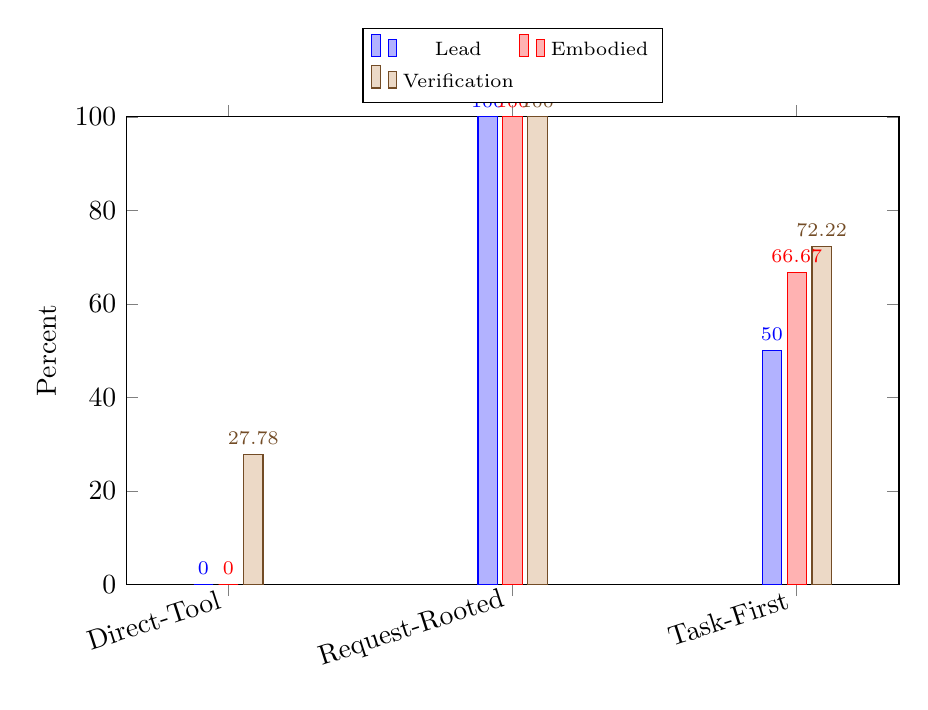
\begin{tikzpicture}
\begin{axis}[
  ybar,
  bar width=7pt,
  width=0.94\columnwidth,
  height=0.62\columnwidth,
  ymin=0,
  ymax=100,
  ylabel={Percent},
  symbolic x coords={Direct-Tool,Request-Rooted,Task-First},
  xtick=data,
  x tick label style={rotate=18, anchor=east},
  legend style={font=\scriptsize, at={(0.5,1.03)}, anchor=south, legend columns=2},
  nodes near coords,
  every node near coord/.append style={font=\scriptsize},
  enlarge x limits=0.18
]
\addplot coordinates {(Direct-Tool, 0) (Request-Rooted, 100) (Task-First, 50)};
\addplot coordinates {(Direct-Tool, 0) (Request-Rooted, 100) (Task-First, 66.66666666666666)};
\addplot coordinates {(Direct-Tool, 27.777777777777775) (Request-Rooted, 100) (Task-First, 72.22222222222221)};
\legend{Lead, Embodied, Verification}
\end{axis}
\end{tikzpicture}
\caption{Outcome quality on the deterministic benchmark. The request-rooted baseline preserves both routing quality and embodied verification fidelity, while the direct-tool baseline collapses on physical-work retention.}
\label{fig:deterministic-benchmark}
\end{figure}


To move beyond authored baselines, we also ran a live-model benchmark through the Boreal web workspace's AI Gateway path using frozen prompt presets, stable local scoring, and recorded request-response metadata \cite{boreal_request_live_benchmark_runner_2026,boreal_request_live_benchmark_results_2026}. The study evaluated five OpenAI-routed models under two prompt families: \emph{neutral\_contract\_v2}, which exposes the output contract without Boreal-specific framing, and \emph{boreal\_canon\_v2}, which adds the request-rooted lead-first rules while keeping the same canonical output vocabulary. The live runner records call success, parse success, exact contract pass, lead accuracy, safe action acceptability, required-role coverage, semantic embodied retention, and semantic verification retention. This split matters because provider access failure, JSON formatting failure, and planning failure are different phenomena and should not be collapsed into one score.

% Generated by apps/web/scripts/run-request-processing-live-benchmark.ts
\begin{table*}[t]
\centering
\small
\setlength{\tabcolsep}{4pt}
\caption{Live request-processing benchmark over frozen prompt presets and real model calls. Exact contract pass remained brittle, so this export emphasizes availability, parse reliability, safe action choice, role preservation, semantic embodied retention, and semantic verification retention.}
\label{tab:live-request-processing-benchmark}
\resizebox{\textwidth}{!}{%
\begin{tabular}{lcccccccccc}
\toprule
System & Call & Parse & Exact Pass & Lead Top-1 & Policy Accept & Required Roles & Exact Embodied & Semantic Embodied & Semantic Verification & False Completion \\
\midrule
gpt-4.1-nano + Neutral & 100.0\% & 75.0\% & 0.0\% & 100.0\% & 100.0\% & 100.0\% & 0.0\% & 83.3\% & 33.3\% & 0.0\% \\
gpt-4.1-nano + Boreal & 100.0\% & 75.0\% & 0.0\% & 100.0\% & 66.7\% & 83.3\% & 0.0\% & 75.0\% & 25.0\% & 0.0\% \\
gpt-5.4-nano + Neutral & 100.0\% & 100.0\% & 0.0\% & 100.0\% & 100.0\% & 87.5\% & 16.7\% & 83.3\% & 33.3\% & 0.0\% \\
gpt-5.4-nano + Boreal & 100.0\% & 100.0\% & 0.0\% & 100.0\% & 100.0\% & 87.5\% & 0.0\% & 100.0\% & 33.3\% & 0.0\% \\
gpt-5-mini + Neutral & 100.0\% & 0.0\% & 0.0\% & n/a & n/a & n/a & n/a & n/a & n/a & n/a \\
gpt-5-mini + Boreal & 100.0\% & 0.0\% & 0.0\% & n/a & n/a & n/a & n/a & n/a & n/a & n/a \\
o4-mini + Neutral & 100.0\% & 50.0\% & 0.0\% & 100.0\% & 100.0\% & 100.0\% & 0.0\% & 100.0\% & 50.0\% & 0.0\% \\
o4-mini + Boreal & 100.0\% & 50.0\% & 0.0\% & 100.0\% & 100.0\% & 100.0\% & 0.0\% & 50.0\% & 0.0\% & 0.0\% \\
gpt-5-pro + Neutral & 0.0\% & 0.0\% & 0.0\% & n/a & n/a & n/a & n/a & n/a & n/a & n/a \\
gpt-5-pro + Boreal & 0.0\% & 0.0\% & 0.0\% & n/a & n/a & n/a & n/a & n/a & n/a & n/a \\
\bottomrule
\end{tabular}
}
\end{table*}


\begin{figure}[t]
\centering
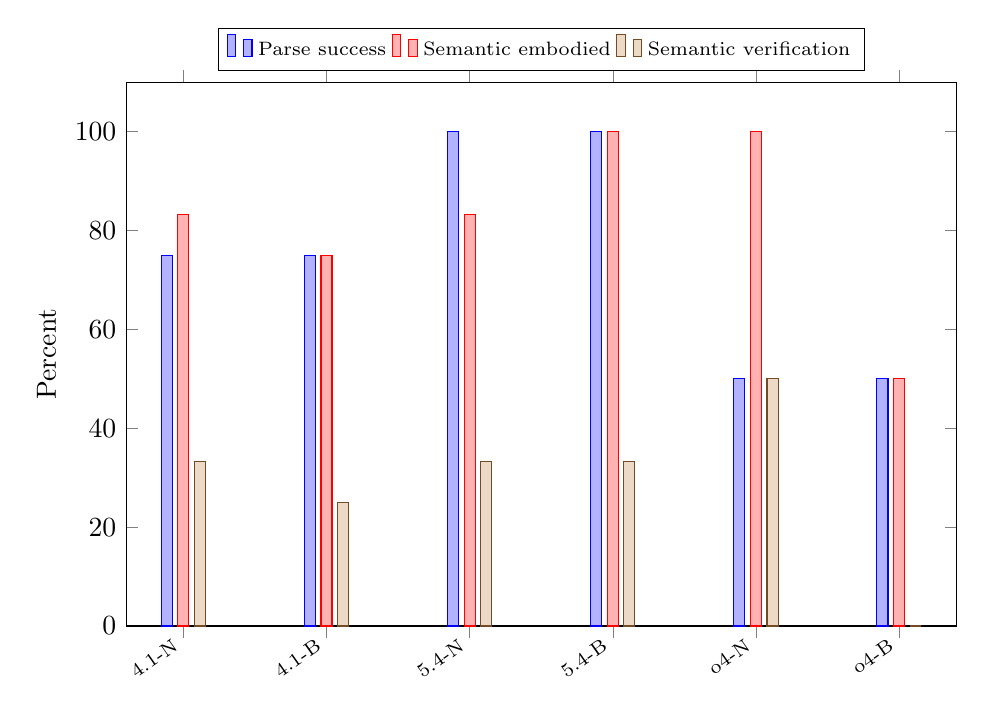
\begin{tikzpicture}
\begin{axis}[
  width=\columnwidth,
  height=0.7\columnwidth,
  ybar,
  bar width=4pt,
  ymin=0,
  ymax=110,
  ylabel={Percent},
  symbolic x coords={4.1-N,4.1-B,5.4-N,5.4-B,o4-N,o4-B},
  xtick=data,
  xticklabel style={rotate=35,anchor=east,font=\scriptsize},
  legend style={font=\scriptsize,at={(0.5,1.02)},anchor=south,legend columns=3},
  enlarge x limits=0.08
]
\addplot coordinates {(4.1-N,75) (4.1-B,75) (5.4-N,100) (5.4-B,100) (o4-N,50) (o4-B,50)};
\addplot coordinates {(4.1-N,83.3) (4.1-B,75) (5.4-N,83.3) (5.4-B,100) (o4-N,100) (o4-B,50)};
\addplot coordinates {(4.1-N,33.3) (4.1-B,25) (5.4-N,33.3) (5.4-B,33.3) (o4-N,50) (o4-B,0)};
\legend{Parse success, Semantic embodied, Semantic verification}
\end{axis}
\end{tikzpicture}
\caption{Live benchmark metrics on the six parsable systems. Labels use model plus prompt family, where N denotes the neutral contract prompt and B denotes the Boreal canon prompt.}
\label{fig:live-normalization-gap}
\end{figure}

The live study reveals a different picture from the deterministic baseline separation. Exact contract pass remains 0\% for every parsable model, which means current models do not reliably emit Boreal's full canonical structured vocabulary even under frozen prompting. However, the strongest parsable systems still show high orchestration competence. GPT-5.4 nano under both prompt families achieved 100\% call success, 100\% parse success, 100\% lead top-1 accuracy, 100\% policy-action acceptability, and 87.5\% required-role coverage. Under the Boreal prompt it also reached 100\% semantic embodied-step recall, though semantic verification completeness remained only 33.3\%. GPT-4.1 nano and o4-mini recovered the correct lead on every parsable scenario but were less reliable structurally, with parse success of 75\% and 50\% respectively. GPT-5 mini returned output on every scenario but never produced valid JSON for the frozen contract, while GPT-5 Pro could not be exercised in this environment because the configured gateway rejected access at call time. We therefore treat GPT-5 Pro as an availability outcome, not as evidence of inferior planning quality.

Figure~\ref{fig:live-normalization-gap} makes the same pattern visible quantitatively. Parse reliability and semantic embodied retention are often materially stronger than semantic verification retention, which suggests that current models can preserve the fact that physical work exists before they can encode the proof obligations that would make that work settlement-safe. The live benchmark therefore sharpens the paper's claim. The main gap is not only whether a model remembers that physical work exists. The stronger gap is whether the model can normalize that knowledge into durable machine-usable execution and verification fields. Current models are already much closer to safe lead selection and false-completion avoidance than to full proof-faithful contract emission. That is exactly the kind of gap a request-rooted durable model can expose.
